%!TEX program = lualatex
% Arquivo: Template_Estat_Texto.tex

\documentclass[a4paper,12pt]{article}

% =========================================================
% Idioma e tipografia (LuaLaTeX)
% =========================================================
\usepackage[portuguese]{babel}
\usepackage{fontspec}
\setmainfont{Latin Modern Roman}

% =========================================================
% Layout
% =========================================================
\usepackage[top=3cm,bottom=2.5cm,left=3cm,right=2.5cm]{geometry}
\usepackage{setspace}
\onehalfspacing
\usepackage{indentfirst}
\setlength{\parindent}{1.25cm}

% =========================================================
% Matemática (align*, etc.)
% =========================================================
\usepackage{amsmath}
\usepackage{amssymb}

% =========================================================
% Tabelas, listas, figuras
% =========================================================
\usepackage{booktabs}
\usepackage{array}
\usepackage{enumitem}
\setlist[itemize]{noitemsep,topsep=3pt}
\setlist[enumerate]{noitemsep,topsep=3pt}

\usepackage{graphicx}
\usepackage{float}
\usepackage{pdflscape}
\graphicspath{{./}{./imagens/}{./figuras/}}

% =========================================================
% Links
% =========================================================
\usepackage{hyperref}
\usepackage{xurl}
\hypersetup{
  colorlinks=true,
  linkcolor=black,
  urlcolor=blue,
  citecolor=black,
  pdfauthor={},
  pdftitle={}
}

% =========================================================
% Texto de preenchimento (lorem)
% =========================================================
\usepackage{lipsum}

% =========================================================
% Dados da capa
% =========================================================
\newcommand{\Instituicao}{Universidade do Estado do Rio de Janeiro}
\newcommand{\Curso}{Física VI -- Oceanografia}
\newcommand{\Professor}{Professor: João Jose}
\newcommand{\Aluno}{Aluno: Israel Oliveira Carneiro\\ Miguel Gayani\\ José Mauro Elsas}
\newcommand{\Cidade}{Rio de Janeiro}
\newcommand{\Ano}{2026}

\title{\textbf{Título do Documento}}
\author{\Aluno}
\date{\Cidade --- \Ano}

\begin{document}

% =========================================================
% Capa (página de rosto)
% =========================================================
\begin{titlepage}
\centering
{\large \Instituicao \par}
\vspace{0.5cm}
{\large \Curso \par}
\vspace{1.0cm}

{\LARGE \textbf{Experimento 1} \par}
\vspace{0.6cm}
{\Large Medidas Elétricas \par}

\begin{figure}[H]
  \centering
  
\includegraphics[width=.3\linewidth]{./uerj.jpg}
\end{figure}

\vfill



\begin{flushright}
\Aluno\\
\Professor
\end{flushright}

\vspace{1.0cm}
{\Cidade --- \Ano \par}
\end{titlepage}


% =========================================================
% Corpo do texto (exemplos)
% =========================================================
\section{Tarefas}

Após realizar a experiência de Medidas Elétricas responda as seguintea questões.

\begin{enumerate}[label=\arabic*--]
    \item Por que as medidas de tensão devem ser iniciadas na maior escala do multímetro?\par\vspace{0.5\baselineskip}
    \emph{Iniciamos as medidas de tensão na maior escala para evitar o risco de sobrecarga no multímetro, protegendo os circuitos das escalas de menor valor.}

    \item Com os dados obtidos no laboratório, preencha a tabela abaixo. \par\vspace{0.5\baselineskip}

    \begin{table}[H]
    \centering
        \begin{tabular}{ccc}
            \toprule
            \shortstack{Posição do\\seletor da fonte} & \shortstack{Tensão Alternada\\(VCA)}& \shortstack{Tensão Contínua \\(VCC)}\\
            \midrule
            1   & 2,1   &2,64\\
            2   & 4,1   &5,53\\
            3   & 6,2   &8,46\\
            4   & 8,3   &11,10\\
            5   & 10,5  &14,35\\
            6   & 12,5  &17,31\\
            7   & 14,7  &20,2\\
            8   & 16,8  &23,1\\
            9   & 18,9  &26,1\\
            10  & 21,0  &29,1\\
            \bottomrule
        \end{tabular}
        \caption{Medidas de VCA e VCC}
        \label{tab:vca_vcc}
\end{table}
\item Usando os dados da tabela \ref{tab:vca_vcc} acima, construa o gráfico da tensão contínua (eixo vertical) em função da corrente alternada (eixo horizontal) e obtenta o coeficiente angular da curva. (OBS: O gráfico pode ser feito em qualquer \textit{software} ou no papel milimetrado).

\begin{figure}[H]
    \centering
    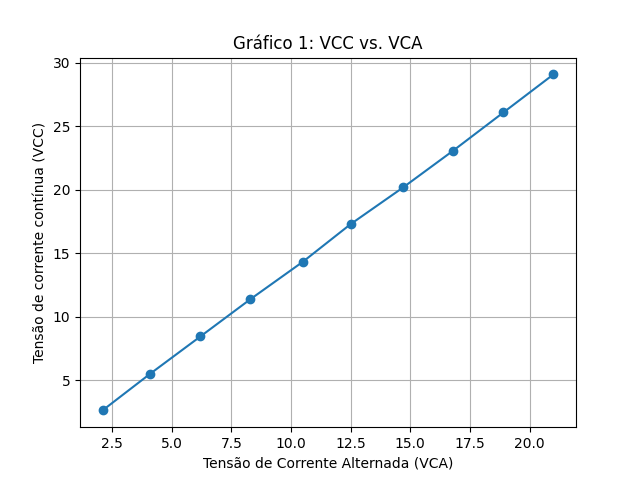
\includegraphics[width=0.8\linewidth]{./Figs/Gráfico_1.png} 
    \caption{Gráfico de Tensão contínua em função da tensão alternada}
    \label{graf:vcc_vca}  
\end{figure}

\subsection{Cálculo do Coeficiente Angular}

O coeficiente angular da reta do gráfico \ref{graf:vcc_vca} é dado por:
\[
    m=\frac{y_2-y_1}{x_2-x_1}
\]
Usando os pontos extremos conforme a tabela \ref{tab:vca_vcc}, temos:
\[
    m=\frac{29,1-2,64}{21,0-2,1}=\frac{26,46}{18,9}=1,4\approx\,\sqrt{2}
\]

    \item Como é possível medir o valor de uma resistência apenas com o multímetro sem uma fonte de energia elétrica. \par\vspace{0.5\baselineskip}

    \emph{Na verdade, deve-se considerar que seja uma medida sem uma fonte externa de energia elétrica. O multímetro tem no seu interior uma pilha que fornece a energia necessária para medir a reistência dentro da faixa adequada de medição. Veja a Figura \ref{fig:multi_dig} abaixo\footnote{ Fonte: https://www.youtube.com/watch?v=zhguLb29z2M}.}

    \begin{figure}[H]
        \centering
        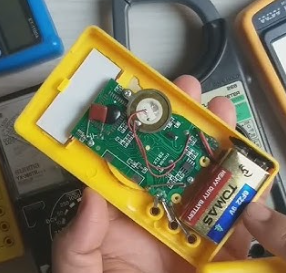
\includegraphics[width=0.65\linewidth]{./Figs/multimetro_bateria.png}
        \caption{Multímetro digital com bateria a vista.}
        \label{fig:multi_dig}
    \end{figure}

    \item Reproduza na tabela abaixo os valores nominal e medido no experimento.

        \begin{table}[H]
    \centering
        \begin{tabular}{cccr}
            \toprule
            \shortstack{Resistores} & \shortstack{Valor\\ Nominal ($\Omega$)}& \shortstack{Valor Medido\\com multímetro digital($\Omega$)}& Diferença ($\epsilon\%$)\\
            \midrule
            R1   & 47    &46,6  &$|-0,9|\implies0,9\%$\\
            R2   & 100   &100   &0,0\%\\
            R3   & 150   &153   &2\%\\
            R4   & 330   &331   &0,3\%\\
            R5   & 470   &473   &0,6\%\\
            \bottomrule
        \end{tabular}
        \caption{Medidas de Resistência Elétrica}
        \label{tab:resistores}
    \end{table}

Então podemos fazer um gráfico \ref{graf:graf_comp} comparativo  direto dos nalores Nominais e dos Valores lidos.

\begin{figure}[H]
    \centering
    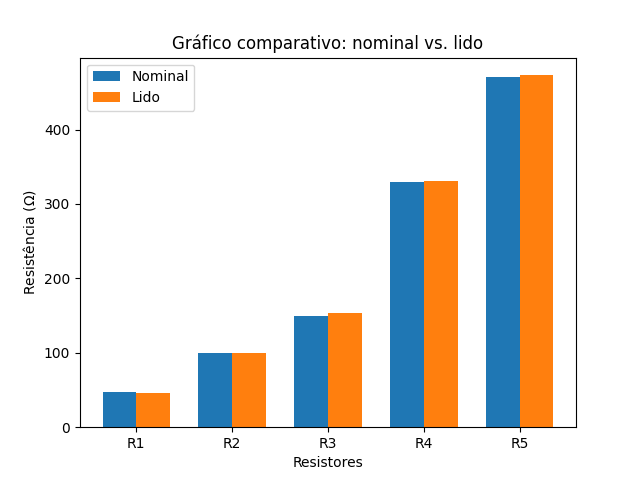
\includegraphics[width=0.6\linewidth]{./Figs/graf_cpmparativo.png}
    \caption{}
    \label{graf:graf_comp}
\end{figure}

\begin{itemize}
    \item Calcule a diferença percentual, usando a expressão abaixo, entre os valores medidos com o multímetro e os valores nominais do fabricante. Considerando que o valor das resistências indicadas pelo fabricante podem variar em até 5\%, as medidas realizadas estão dentro da precisão especificada pelo fabricante.
    
    Pata calcular o erro $\epsilon\%$ foi usada a fórmula:

    \[
        \epsilon\%=\frac{|R_{medido}-R_{nominal}|}{R_{nominal}}
    \]

    \emph{Assim temos:}
    \begin{figure}[H]
        \centering
        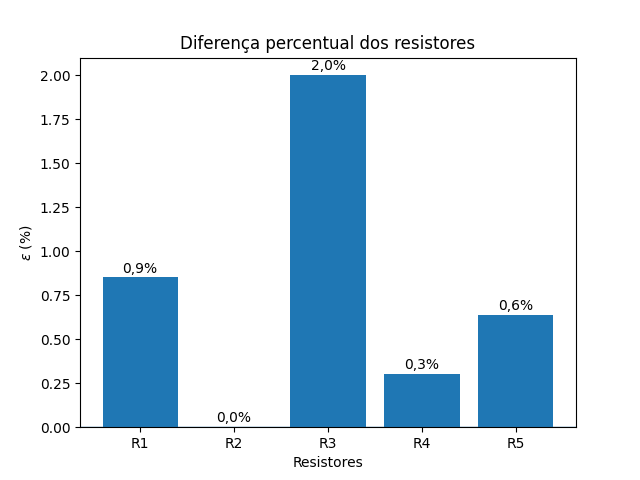
\includegraphics[width=0.6\linewidth]{./Figs/graf_cpmparativo_2.png}
    \end{figure}
\end{itemize}
\end{enumerate}
\end{document}